\documentclass[12pt]{article}
\usepackage[margin=1in]{geometry}
\usepackage{graphicx}
\usepackage{amsmath}
\usepackage{tikz}
\usepackage{hyperref}
\usepackage{enumitem}
\usepackage{mathtools}

\newcommand{\dlo}{d_{L_1}}
\newcommand{\dlt}{d_{L_2}}
\newcommand{\dlot}{d_{12}}

\newcommand{\xpy}[2]{\prescript{#1}{}{P}_{#2}}
\newcommand{\rxpy}[2]{{\color{red} \prescript{#1}{}{P}_{#2}}}
\newcommand{\gxpy}[2]{{\color{green} \prescript{#1}{}{P}_{#2}}}
\newcommand{\bxpy}[2]{{\color{blue} \prescript{#1}{}{P}_{#2}}}

\newcommand{\xoy}[2]{\prescript{#1}{}{\theta}_{#2}}
\newcommand{\rxoy}[2]{{\color{red} \prescript{#1}{}{\theta}_{#2}}}
\newcommand{\gxoy}[2]{{\color{green} \prescript{#1}{}{\theta}_{#2}}}
\newcommand{\bxoy}[2]{{\color{blue} \prescript{#1}{}{\theta}_{#2}}}

\newcommand{\xcy}[2]{\prescript{#1}{}{C}_{#2}}
\newcommand{\rxcy}[2]{{\color{red} \prescript{#1}{}{C}_{#2}}}
\newcommand{\gxcy}[2]{{\color{green} \prescript{#1}{}{C}_{#2}}}
\newcommand{\bxcy}[2]{{\color{blue} \prescript{#1}{}{C}_{#2}}}

\newcommand{\xmle}{\hat{x}^{MLE}_k}
\newcommand{\amax}{\underset{x}{\mathrm{argmax}}}
\newcommand{\amin}{\underset{x}{\mathrm{argmin}}}
\newcommand{\amingpr}{\underset{\xpy{G}{R}}{\mathrm{argmin}}}

\newcommand{\pde}[2]{\frac{\partial #1}{\partial #2}}

\title{CSCI 5552 - HW1}
\author{Yashasvi Sriram Patkuri\\patku001@umn.edu}

\begin{document}
\maketitle
\pagebreak

\section{}
3D static robot

Known variables: global relative positions of landmarks $ \gxpy{G}{L_1}, \gxpy{G}{L_2} $.

Measured variables: relative positions of landmarks from robot {\color{blue} $ \bxpy{R}{L_1}, \bxpy{R}{L_2} $ }

Required variables: global relative position and orientation of the robot {\color{red} $ \rxpy{G}{R}, \rxcy{G}{R} $ }

Then we have the following relations

\[
  \gxpy{G}{L_1} \equiv \rxpy{G}{R} + \rxcy{G}{R} * \bxpy{R}{L_1}
\]
\[
  \gxpy{G}{L_2} \equiv \rxpy{G}{R} + \rxcy{G}{R} * \bxpy{R}{L_2}
\]
\subsection*{1 measurement}
Given a single measurement the possible set of positions of the robot is a sphere with center as the position of landmark.
For each of the possible positions if the robot frame is rotated arbitrarily along the vector from its origin to the landmark still the measurements will be the same.
Therefore each possible position has infinitely many possible orientations.

\subsection*{2 measurements}
When one more measurement is received the possible positions of robot becomes the intersection of two spheres formed by each landmark measurement, i.e. it is a circle.
This circle of intersection of two spheres has its center on the line joining the centers of the spheres.
The normal to the circle is given by (from notes, lecture 8)
\[
  {\color{green} \prescript{G}{}{\hat{n}}_{12}} \equiv \frac{\gxpy{G}{L_1} - \gxpy{G}{L_2}}{\Vert \gxpy{G}{L_1} - \gxpy{G}{L_2} \Vert}
\]

To get the center of the circle, consider a triangle with vertices as $ \gxpy{G}{L_1}, \gxpy{G}{L_2}  $ and some point on circle.
\begin{figure}[h!]
  \centering
  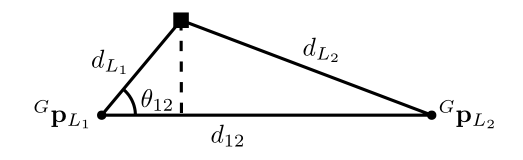
\includegraphics[width=0.8\textwidth]{1.png}
  \caption{Triangle}
  \label{fig:1}
\end{figure}

All the distances are known in the figure \ref{fig:1}, so we can solve for $\theta_{12}$.
\[
  \dlt^2 = \dlo^2 + \dlot^2 - 2 * \dlo * \dlot * cos(\theta_{12})
\]
\[
  \theta_{12} = acos(\frac{\dlt^2 - \dlo^2 - \dlot^2}{-2\dlo\dlot})
\]

Then we have the radius and center of the circle as
\[
  r = \dlo * sin(\theta_{12})
\]
\[
  \bxpy{G}{12}^c = \gxpy{G}{L_1} + \dlo cos(\theta_{12}) \prescript{G}{}{\hat{n}}_{12}
\]
Concisely
\[
  \Vert \xpy{G}{R} - \xpy{G}{12}^c \Vert = r
\]
\[
  (\xpy{G}{R} - \xpy{G}{12}^c)^T * \prescript{G}{}{\hat{n}}_{12} = 0
\]

Therefore we have the equation of the circle of possible positions.
Each point on this circle has a single valid orientation.

\subsection*{determining position}
In general as the possible set of positions of the robot is a circle (which contains infinitely many points) and hence the position cannot be determined uniquely.
But in the limiting cases where the intersection of the spheres is a point, we can determine the position of the robot.
This can happen in two way, two sphere touching each other from outside or one sphere inside another sphere touching at one point as illustrated in figure \ref{fig:2}.

\def\ringa{(0,0) circle (2)}
\def\ringb{(3,0) circle (1)}
\def\ringc{(5,0) circle (2)}
\def\ringd{(6,0) circle (1)}

\begin{figure}[h]
  \centering
  \begin{tikzpicture}
      \node[draw,circle,inner sep=1pt,fill] at (0, 0) {};
      \node[draw,inner sep=2pt,fill] at (2, 0) {};
      \node[draw,circle,inner sep=1pt,fill] at (3, 0) {};
      \draw \ringa;
      \draw \ringb;
  \end{tikzpicture}
  \begin{tikzpicture}
      \node[draw,circle,inner sep=1pt,fill] at (5, 0) {};
      \node[draw,circle,inner sep=1pt,fill] at (6, 0) {};
      \node[draw,inner sep=2pt,fill] at (7, 0) {};
      \draw \ringc;
      \draw \ringd;
  \end{tikzpicture}
  \caption{Touching spheres}
  \label{fig:2}
\end{figure}
For both cases we shall have the necessary and sufficient condition that $ L_1, L_2, R $ are collinear. In other words
\[
  \bxpy{R}{L_1} = \alpha * \bxpy{R}{L_2}
\]
for some real $\alpha$.
The point of touching can be found by translating from first landmark $ \gxpy{G}{L_1} $ by a distance of $ \Vert \bxpy{R}{L_1} \Vert $ in the direction of the other landmark $ \frac{\gxpy{G}{L_2} - \gxpy{G}{L_1}}{\Vert \gxpy{G}{L_2} - \gxpy{G}{L_1} \Vert} $. Therefore
\[
  \xpy{G}{R} = \gxpy{G}{L_1} + \frac{\gxpy{G}{L_2} - \gxpy{G}{L_1}}{\Vert \gxpy{G}{L_2} - \gxpy{G}{L_1} \Vert} * \Vert \bxpy{R}{L_1} \Vert
\]

\subsection*{determining orientation for these positions?}
Orientation cannot be determined in the limiting cases.
For these limiting cases, there are infinitely many orientations possible.
This can be proved using proof as follows.

As we have seen that the necessary and sufficient condition for the limiting case is that $L_1, L_2, R$ are collinear.
So we can imagine an axis that passes through origin of robot frame and $ L_1, L_2 $.
If we rotate the robot frame around this axis by some finite amount, the measurements $ \bxpy{R}{L_1}, \bxpy{R}{L_2} $ do not change.
In other words given the measurements we cannot disambiguate b/w two orientations of the robot.
There is no additional information to reduce number of possible orientations.
And as the rotation is arbitrary there can be infinitely many possible orientations for given measurements $ \bxpy{R}{L_1}, \bxpy{R}{L_2} $.
Therefore the orientation of robot cannot be uniquely determined in the limiting cases.

\pagebreak

\section{}
2D moving robot

Known variables: global relative positions of landmarks $ \gxpy{G}{L_1}, \gxpy{G}{L_2} $ and odometry b/w two robot poses {\color{green} $ \gxpy{R_1}{R_2}, \gxoy{R_1}{R_2} $ }

Measured variables: relative positions of one landmark from each pose of robot {\color{blue} $ \bxpy{R_1}{L_1}, \bxpy{R_2}{L_2} $ }

Required variables: global relative positions and orientations of both configurations of the robot {\color{red} $ \rxpy{G}{R_1}, \rxoy{G}{R_1}, \rxpy{G}{R_2}, \rxoy{G}{R_2} $}

Then we have the following relations

\[
  \gxpy{G}{L_1} \equiv \rxpy{G}{R_1} + \rxoy{G}{R_1} * \bxpy{R_1}{L_1}
\]
\[
  \gxpy{G}{L_2} \equiv \rxpy{G}{R_1} + \rxoy{G}{R_1} * \xpy{R_1}{L_2}
\]

We do not have access to $ \xpy{R_1}{L_2} $. But we do have $ \xpy{R_2}{L_2} $ and odometry, therefore we can write

\[
  \xpy{R_1}{L_2} \equiv \gxpy{R_1}{R_2} + \gxoy{R_1}{R_2} * \bxpy{R_2}{L_2}
\]
\[
  \gxpy{G}{L_2} \equiv \rxpy{G}{R_1} + \rxoy{G}{R_1} * (\gxpy{R_1}{R_2} + \gxoy{R_1}{R_2} * \bxpy{R_2}{L_2})
\]

Therefore we have a system of linear equations with 2 ($\xpy{G}{R_1}$) + 1-ish ($\xoy{G}{R_1}$) variables and 4 equations. More importantly this has the same form as solving for robot pose using 2 relative position measurements in 2D (notes, lecture 6).
\[
  \gxpy{G}{L_1} \equiv \rxpy{G}{R_1} + \rxoy{G}{R_1} * \bxpy{R_1}{L_1}
\]
\[
  \gxpy{G}{L_2} \equiv \rxpy{G}{R_1} + \rxoy{G}{R_1} * (\gxpy{R_1}{R_2} + \gxoy{R_1}{R_2} * \bxpy{R_2}{L_2})
\]

Subtracting the above two equations so that $ \rxpy{G}{R_1} $ cancels out, we have
\[
  \gxpy{G}{L_1} - \gxpy{G}{L_2} \equiv \rxoy{G}{R_1} * \bxpy{R_1}{L_1} - \rxoy{G}{R_1} * (\gxpy{R_1}{R_2} + \gxoy{R_1}{R_2} * \bxpy{R_2}{L_2})
\]
Simplifying we get
\[
  \gxpy{G}{L_1} - \gxpy{G}{L_2} \equiv \rxoy{G}{R_1} * (\bxpy{R_1}{L_1} - \gxpy{R_1}{R_2} - \gxoy{R_1}{R_2} * \bxpy{R_2}{L_2})
\]
As this is all in 2D $ \gxpy{G}{L_1} - \gxpy{G}{L_2}, \rxoy{G}{R_1}, \bxpy{R_1}{L_1} - \gxpy{R_1}{R_2} - \gxoy{R_1}{R_2} * \bxpy{R_2}{L_2} $ are 2 x 1, 2 x 2 and 2 x 1 matrices respectively. Let

\[
  \gxpy{G}{L_1} - \gxpy{G}{L_2} \equiv \begin{bmatrix} \gxpy{G}{L12_{x}} \\ \gxpy{G}{L12_{y}} \end{bmatrix}
\]

\[
  \bxpy{R_1}{L_1} - \gxpy{R_1}{R_2} - \gxoy{R_1}{R_2} * \bxpy{R_2}{L_2} \equiv \begin{bmatrix} \bxpy{R}{x} \\ \bxpy{R}{y} \end{bmatrix}
\]

\[
  \rxoy{G}{R_1} \equiv \begin{bmatrix} cos(\rxoy{G}{R_1}) & -sin(\rxoy{G}{R_1}) \\ sin(\rxoy{G}{R_1}) & cos(\rxoy{G}{R_1}) \end{bmatrix}
\]

Substituting new expressions in the previous equation gives

\[
\begin{bmatrix} \gxpy{G}{L12_{x}} \\ \gxpy{G}{L12_{y}} \end{bmatrix}
  \equiv
  \begin{bmatrix} cos(\rxoy{G}{R_1}) & -sin(\rxoy{G}{R_1}) \\ sin(\rxoy{G}{R_1}) & cos(\rxoy{G}{R_1}) \end{bmatrix}
  *
  \begin{bmatrix} \bxpy{R}{x} \\ \bxpy{R}{y} \end{bmatrix}
\]

\[
\begin{bmatrix} \gxpy{G}{L12_{x}} \\ \gxpy{G}{L12_{y}} \end{bmatrix}
  \equiv
  \begin{bmatrix} \bxpy{R}{x} * cos(\rxoy{G}{R_1}) - \bxpy{R}{y} * sin(\rxoy{G}{R_1}) \\ \bxpy{R}{x} * sin(\rxoy{G}{R_1}) + \bxpy{R}{y} * cos(\rxoy{G}{R_1}) \end{bmatrix}
\]

\[
\begin{bmatrix} \gxpy{G}{L12_{x}} \\ \gxpy{G}{L12_{y}} \end{bmatrix}
  \equiv
  \begin{bmatrix} \bxpy{R}{x} & -\bxpy{R}{y} \\ \bxpy{R}{y} & \bxpy{R}{x} \end{bmatrix}
  *
  \begin{bmatrix} cos(\rxoy{G}{R_1}) \\ sin(\rxoy{G}{R_1}) \end{bmatrix}
\]

This is a system of linear equations in cosine and sine of required $ \rxoy{G}{R_1} $ and everything else is either known or measured, so we can solve by taking the left inverse

\[
\begin{bmatrix} cos(\rxoy{G}{R_1}) \\ sin(\rxoy{G}{R_1}) \end{bmatrix}
  \equiv
  \begin{bmatrix} \bxpy{R}{x} & -\bxpy{R}{y} \\ \bxpy{R}{y} & \bxpy{R}{x} \end{bmatrix}^{-1}
  *
  \begin{bmatrix} \gxpy{G}{L12_{x}} \\ \gxpy{G}{L12_{y}} \end{bmatrix}
\]

Using the defintion of 2D matrix inverse we have

\[
\begin{bmatrix} cos(\rxoy{G}{R_1}) \\ sin(\rxoy{G}{R_1}) \end{bmatrix}
  \equiv
  \frac{1}{\bxpy{R}{x}^2 + \bxpy{R}{y}^2}
  *
  \begin{bmatrix} \bxpy{R}{x} & \bxpy{R}{y} \\ -\bxpy{R}{y} & \bxpy{R}{x} \end{bmatrix}
  *
  \begin{bmatrix} \gxpy{G}{L12_{x}} \\ \gxpy{G}{L12_{y}} \end{bmatrix}
\]

\subsection*{unsolvable case}
The inverse exists iff $ \bxpy{R}{x}^2 + \bxpy{R}{y}^2 \neq 0 $.
As $ \bxpy{R}{x}, \bxpy{R}{y} $ represent columns of $ \bxpy{R_1}{L_1} - \gxpy{R_1}{R_2} - \gxoy{R_1}{R_2} * \bxpy{R_2}{L_2} $, which is nothing but $ \bxpy{R_1}{L_1} - \bxpy{R_1}{L_2} $, the condition for inverse existence is equivalent to saying that distance b/w $ L_1 and L_2 \neq 0 $.
Simply put the inverse does not exists iff $ L_1, L_2 $ are at same points in space.

From the cosine and sine of $ \rxoy{G}{R_1} $ we can get $ \rxoy{G}{R_1} $ using atan2 function
\[
  \rxoy{G}{R_1} \equiv atan2(sin(\rxoy{G}{R_1}), cos(\rxoy{G}{R_1}))
\]

Putting this back into the initial equations, now with calculated $ \bxoy{G}{R_1} $
\[
  \gxpy{G}{L_1} \equiv \rxpy{G}{R_1} + \bxoy{G}{R_1} * \bxpy{R_1}{L_1}
\]
\[
  \gxpy{G}{L_2} \equiv \rxpy{G}{R_1} + \bxoy{G}{R_1} * (\gxpy{R_1}{R_2} + \gxoy{R_1}{R_2} * \bxpy{R_2}{L_2})
\]

Adding the above two equations and making $ \rxpy{G}{R_1} $ the subject we have
\[
  \rxpy{G}{R_1} \equiv \frac{1}{2} * [(\gxpy{G}{L_1} + \gxpy{G}{L_2}) - \bxoy{G}{R_1} * (\bxpy{R_1}{L_1} + \gxpy{R_1}{R_2} + \gxoy{R_1}{R_2} * \bxpy{R_2}{L_2})]
\]

Now that we have calculated $ \bxpy{G}{R_1} $ we can use the following equation to get $ \rxpy{G}{R_2} $

\[
  \rxpy{G}{R_2} \equiv \bxpy{G}{R_1} + \bxoy{G}{R_1} * \gxpy{R_1}{R_2}
\]

We can use the following equation to calculate $ \rxoy{G}{R_2} $ using $ \bxoy{G}{R_1} $

\[
  \rxoy{G}{R_2} \equiv \bxoy{G}{R_1} * \gxoy{R_1}{R_2}
\]

All the required quantities are calculated and the only case where the solution is impossible to calculate is when both landmarks $ L_1, L_2 $ lie on same point in space.
\pagebreak

\section{}

\subsection*{3.a}
Given robot can measure
\[
  {\color{blue} d_L_i} \equiv \hat{\gxpy{G}{L_i}}^T * \rxpy{G}{R} + n_i,\ s.t.\ n_i \sim N(0, \sigma_i)
\]
Green quantities are known, blue quantities are measured and red quantities are unknown and required.

As the above equation is a dot product of unknown vector with a known unit vector, the equation is linear in $ \rxpy{G}{R} $.
Therefore we can model this as a linear weighted estimation problem.

Consider
\[
  z_i \equiv H_i * x + n_i, s.t. n_i \sim N(0, \sigma_i)
\]

The maximum likelihood estimation method tries to find the $x$ that maximizes the joint probability distribution of required value and evidence. i.e.
\[
  \xmle \equiv \amax\ p(x, z_1, z_2, ... z_k)
\]

Assuming all measurements are independent we have
\[
  \xmle \equiv \amax\ p(x, z_1, z_2, ... z_k) \equiv \amax\ \prod_{i=1}^{k} p(x, z_i)
\]

But as $n_i$ follows a normal distribution with mean = 0 and standard deviation = $\sigma_i$, we know for an n-dimensional value x
\[
  p(x, z_i) \equiv \frac{1}{(2\pi)^{n/2}|\Sigma_i|^{1/2}} e^{-\frac{1}{2} (H_ix - z_i)^T\Sigma_i^{-1}(H_ix - z_i)}
\]

Therefore we have
\[
  \xmle \equiv \amax\ \prod_{i=1}^{k} \frac{1}{(2\pi)^{n/2}|\Sigma_i|^{1/2}} e^{-\frac{1}{2} (H_ix - z_i)^T\Sigma_i^{-1}(H_ix - z_i)}
\]

To maximize this function directly is cumbersome, therefore we maximize the log of this.
The maximum of log of the function occurs at the same value as the maximum of function itself.
This is because log is monotonic and does not flip sign.
\[
  \xmle \equiv \amax\ log(\prod_{i=1}^{k} \frac{1}{(2\pi)^{n/2}|\Sigma_i|^{1/2}} e^{-\frac{1}{2} (H_ix - z_i)^T\Sigma_i^{-1}(H_ix - z_i)})
\]

This simplifies further
\[
  \xmle \equiv \amax\ \sum_{i=1}^{k} log(\frac{1}{(2\pi)^{n/2}|\Sigma_i|^{1/2}} e^{-\frac{1}{2} (H_ix - z_i)^T\Sigma_i^{-1}(H_ix - z_i)})
\]
\[
  \xmle \equiv \amax\ \sum_{i=1}^{k} log(\frac{1}{(2\pi)^{n/2}|\Sigma_i|^{1/2}}) + log(e^{-\frac{1}{2} (H_ix - z_i)^T\Sigma_i^{-1}(H_ix - z_i)})
\]
\[
  \xmle \equiv \amax\ \sum_{i=1}^{k} {\color{red} log(\frac{1}{(2\pi)^{n/2}|\Sigma_i|^{1/2}})} -\frac{1}{2} (H_ix - z_i)^T\Sigma_i^{-1}(H_ix - z_i)
\]
using log algebra rules.

The term in red does not depend on x, therefore the argmax of the above function is the same as the argmax of the other term.
Hence we have
\[
  \xmle \equiv {\color{blue} \amax\ \sum_{i=1}^{k} -\frac{1}{2} (H_ix - z_i)^T\Sigma_i^{-1}(H_ix - z_i)}
\]

\paragraph{Note}
By taking the minus sign out we can convert this to a weighed linear least squares problem.
But as this is linear in required variable x, we can get closed form or analytical solution for this directly.

To maximum the function we need x where gradient = 0 and hessian $<$ 0 (notes, lecture 3).

Setting gradient of function in blue = 0 gives
\[
  \sum_{i=1}^{k} -(H_i^T * \Sigma_i^{-1} * H_i) * x + (H_i^T * \Sigma_i^{-1} * z_i) = 0
\]
which gives
\[
  {\color{blue} \sum_{i=1}^{k} (H_i^T * \Sigma_i^{-1} * H_i)}  * x = {\color{blue} \sum_{i=1}^{k} (H_i^T * \Sigma_i^{-1} * z_i)}
\]
Everything in blue is known, therefore we can solve for x by taking left inverse
\[
  x = {\color{blue} (\sum_{i=1}^{k} H_i^T * \Sigma_i^{-1} * H_i)}^{-1} * {\color{blue} \sum_{i=1}^{k} (H_i^T * \Sigma_i^{-1} * z_i)}
\]
Of course this is only possible to calculate if inverse of $ \sum_{i=1}^{k} (H_i^T * \Sigma_i^{-1} * H_i) $ exists.

To show that this is really the maximum we need to show the hessian $<$ 0.
So taking double derivative of the function we get
\[
  \nabla^2_x p(x, z_1, z_2, ... z_k) \equiv \nabla_x (\sum_{i=1}^{k} -(H_i^T * \Sigma_i^{-1} * H_i) * x + (H_i^T * \Sigma_i^{-1} * z_i))
\]
\[
  \nabla^2_x p(x, z_1, z_2, ... z_k) \equiv \sum_{i=1}^{k} -H_i^T * \Sigma_i^{-1} * H_i
\]
\[
  \nabla^2_x p(x, z_1, z_2, ... z_k) \equiv \sum_{i=1}^{k} -H_i^T * \Sigma_i^{-1} * H_i < 0, \text{when $\Sigma_i$ is positive definite, which it is}
\]

Therefore the above calculated x is the argmax and hence the required maximum likelihood estimate
\[
  \xmle \equiv {\color{blue} (\sum_{i=1}^{k} H_i^T * \Sigma_i^{-1} * H_i)}^{-1} * {\color{blue} \sum_{i=1}^{k} (H_i^T * \Sigma_i^{-1} * z_i)}
\]

In this case we have
\[
  H_i \equiv (\frac{\gxpy{G}{L_i}}{\Vert\gxpy{G}{L_i}\Vert})^T
\]
\[
  z_i \equiv {\color{blue} d_L_i}
\]
\[
  x_i \equiv \rxpy{G}{R}
\]
\[
  \Sigma_i \equiv \sigma_i^2
\]

Substituting these terms into general formula
\[
  \rxpy{G}{R}
  \equiv
  {\color{blue}
    (\sum_{i=1}^{k} \frac{\gxpy{G}{L_i}}{\Vert\gxpy{G}{L_i}\Vert} * \sigma_i^{-2} * (\frac{\gxpy{G}{L_i}}{\Vert\gxpy{G}{L_i}\Vert})^T)^{-1}
    *
    \sum_{i=1}^{k} (\frac{\gxpy{G}{L_i}}{\Vert\gxpy{G}{L_i}\Vert} * \sigma_i^{-2} * d_L_i)
  }
\]
which simplifies to the following as $\Sigma_i$ in our case is a scalar
\[
  \rxpy{G}{R}
  \equiv
  {\color{blue}
    (\sum_{i=1}^{k} \frac{1}{\sigma_i^2} * (\frac{\gxpy{G}{L_i}}{\Vert\gxpy{G}{L_i}\Vert}) * (\frac{\gxpy{G}{L_i}}{\Vert\gxpy{G}{L_i}\Vert})^T )^{-1}
    *
    \sum_{i=1}^{k} ( \frac{1}{\sigma_i^2} * \frac{\gxpy{G}{L_i}}{\Vert\gxpy{G}{L_i}\Vert} * d_L_i )
  }
\]
The first term has order 2 x 2, second term has 2 x 1 and therefore we have order of $\rxpy{G}{R}$ as 2 x 1 which checks out.
\pagebreak

\subsection*{3.c}
Given robot can measure
\[
  {\color{blue} d_L_i} \equiv \Vert\rxpy{G}{R} - \gxpy{G}{L_i}\Vert + n_i,\ s.t.\ n_i \sim N(0, \sigma_i)
\]
Green quantities are known, blue quantities are measured and red quantities are unknown and required.

As the above equation is a euclidean distance from a landmark, the equation is non-linear in $ \rxpy{G}{R} $.
Therefore we can model this as a non-linear weighted estimation problem.

Consider
\[
  z_i \equiv h_i(x) + n_i, s.t. n_i \sim N(0, \sigma_i)
\]

We follow the similar logic as in 3.a to arrive at the equation
\[
  \xmle \equiv \amax\ \sum_{i=1}^{k} -\frac{1}{2} (h_i(x) - z_i)^T\Sigma_i^{-1}(h_i(x) - z_i)
\]

Taking the - sign and half out we have a minimization problem
\[
  \xmle \equiv \amin\ \sum_{i=1}^{k} (h_i(x) - z_i)^T\Sigma_i^{-1}(h_i(x) - z_i)
\]

In this case we have (assuming 3D analysis)
\[
  h_i \equiv \Vert\xpy{G}{R} - \gxpy{G}{L_i}\Vert \equiv \sqrt{ (x - x_L_i)^2 + (y - y_L_i)^2 + (z - z_L_i)^2 }
\]
\[
  z_i \equiv {\color{blue} d_L_i}
\]
\[
  x_i \equiv \rxpy{G}{R}
\]
\[
  \Sigma_i \equiv \sigma_i^2
\]

So substituting we get
\[
  \hat{\rxpy{G}{R}} \equiv \amingpr\ \sum_{i=1}^{k} (\Vert\xpy{G}{R} - \gxpy{G}{L_i}\Vert - {\color{blue} d_L_i})^T\sigma_i^{-2}(\Vert\xpy{G}{R} - \gxpy{G}{L_i}\Vert - {\color{blue} d_L_i})
\]

Also $ \Sigma_i $ is a scalar,
\[
  \hat{\rxpy{G}{R}}
    \equiv
  \amingpr\
    \sum_{i=1}^{k} \sigma_i^{-2} * (\Vert\xpy{G}{R} - \gxpy{G}{L_i}\Vert - {\color{blue} d_L_i})^T * (\Vert\xpy{G}{R} - \gxpy{G}{L_i}\Vert - {\color{blue} d_L_i})
\]
\[
  \hat{\rxpy{G}{R}}
    \equiv
  \amingpr\
  \sum_{i=1}^{k} \frac{1}{\sigma_i^2} * \Vert\Vert\xpy{G}{R} - \gxpy{G}{L_i}\Vert - {\color{blue} d_L_i}\Vert^2
\]
Hence this estimation problem is a non-linear weighted least squares problem with
\[
  \sum_{i=1}^{k} \frac{1}{\sigma_i^2} * \Vert\Vert\xpy{G}{R} - \gxpy{G}{L_i}\Vert - {\color{blue} d_L_i}\Vert^2
\]
as loss function.

\subsection*{first order taylor approximation}
For any $h_i(x)$ we have
\[
  h_i(X) \approx h_i(\hat{X}) + J(h_i(X)) |_{X = \hat{X}} * (X - \hat{X})
\]
where \hat{x} is an initial guess and J is Jacobian of the field.

Assuming our distance function which is actually a scalar field is in 3D,
\[
  J(h_i(X))|_{X = \hat{X}}
  \equiv
  \begin{bmatrix} \pde{h_i}{x}|_{X = \hat{X}} &  \pde{h_i}{y} |_{X = \hat{X}} & \pde{h_i}{z} |_{X = \hat{X}} \end{bmatrix}
\]
Consider
\[
  \pde{h_i}{x}|_{X = \hat{X}} = \pde{\sqrt{ (x - x_L_i)^2 + (y - y_L_i)^2 + (z - z_L_i)^2 }}{X}|_{x = \hat{X}}
\]
\[
  \pde{h_i}{x}|_{X = \hat{X}} = \frac{2 * (x - x_L_i)}{2 * \sqrt{ (x - x_L_i)^2 + (y - y_L_i)^2 + (z - z_L_i)^2 }}|_{X = \hat{X}}
\]
\[
  \pde{h_i}{x}|_{X = \hat{X}} = \frac{\hat{x} - x_L_i}{h_i(\hat{X})}
\]
Partial derivatives w.r.t to y and z will have the same form.
Therefore we have,
\[
  J(h_i(X))|_{X = \hat{X}}
  \equiv
  \begin{bmatrix} \frac{\hat{x} - x_L_i}{h_i(\hat{X})} & \frac{\hat{y} - y_L_i}{h_i(\hat{X})} & \frac{\hat{z} - z_L_i}{h_i(\hat{X})} \end{bmatrix}
  \equiv
  \frac{1}{h_i(\hat{X})} * \begin{bmatrix} \hat{x} - x_L_i & \hat{y} - y_L_i & \hat{z} - z_L_i \end{bmatrix}
\]
\[
  J(h_i(X))|_{X = \hat{X}}
  \equiv
  \frac{1}{h_i(\hat{X})} * (\hat{X} - \gxpy{G}{L_i})^T
\]

Therefore first order approximation is
\[
  h_i(X) \approx h_i(\hat{X}) + \frac{1}{h_i(\hat{X})} * (\hat{X} - \gxpy{G}{L_i})^T * (X - \hat{X})
\]
\[
  h_i(X) \approx \Vert \hat{X} - \gxpy{G}{L_i} \Vert + (\frac{\hat{X} - \gxpy{G}{L_i}}{\Vert \hat{X} - \gxpy{G}{L_i} \Vert})^T * (X - \hat{X})
\]

\subsection*{iterative solve}
Using this approximation we have least squares cost function as
\[
  \hat{\rxpy{G}{R}}
    \equiv
  \amingpr\
  \sum_{i=1}^{k}
    \frac{1}{\sigma_i^2}
    *
    \Vert
      {\color{blue} d_L_i}
      - \Vert \hat{X} - \gxpy{G}{L_i} \Vert
      - (\frac{\hat{X} - \gxpy{G}{L_i}}{\Vert \hat{X} - \gxpy{G}{L_i} \Vert})^T * (X - \hat{X})
    \Vert^2
\]
or
\[
  \hat{\rxpy{G}{R}}
    \equiv
  \amingpr\
  \sum_{i=1}^{k}
    \frac{1}{\sigma_i^2}
    *
    \Vert
      r_i
      - H_i * (X - \hat{X})
    \Vert^2
\]
where $ r_i \equiv {\color{blue} d_L_i} - \Vert \hat{X} - \gxpy{G}{L_i} \Vert $ and $ H_i \equiv (\frac{\hat{X} - \gxpy{G}{L_i}}{\Vert \hat{X} - \gxpy{G}{L_i} \Vert})^T $

For this form we have (from notes, lecture 5) the following minimization algorithm
\[
  X = \hat{X} + (\sum_{i = 1}^k \frac{1}{\sigma_i^2} * H_i^T * H_i)^{-1} * (\sum_{i = 1}^k \frac{1}{\sigma_i^2} * H_i^T * r_i)
\]
where $ r_i \equiv {\color{blue} d_L_i} - \Vert \hat{X} - \gxpy{G}{L_i} \Vert $ and $ H_i \equiv (\frac{\hat{X} - \gxpy{G}{L_i}}{\Vert \hat{X} - \gxpy{G}{L_i} \Vert})^T, X \equiv \rxpy{G}{R} $

Therefore by taking an initial guess $ \hat{\xpy{G}{R}} $ and solving for $ \xpy{G}{R} $ recursively we can get better and better estimates of $ \rxpy{G}{R} $.

\end{document}
